\documentclass{beamer}
\setbeamertemplate{section in toc}[sections numbered]

\usepackage[utf8]{inputenc}
\usepackage[croatian]{babel}
\usepackage[T1]{fontenc}
\usepackage{lmodern}

\usepackage{mathtools}
\usepackage{listings}
\usepackage{tikz-uml}
\usepackage{multirow}
\usepackage{tikz}
\usepackage{svg}

\usetheme[numbering=fraction]{metropolis}

\title{Sybil napadi u društvenim mrežama i zaštita od njih}
\author{Antun Razum\\Voditelj: prof. dr. sc. Siniša Srbljić}
\institute{Fakultet elektrotehnike i računarstva}
\date{\today}

\begin{document}

\maketitle

\begin{frame}{Sadržaj}
  \tableofcontents
\end{frame}

\section{Uvod}

\begin{frame}{Sybil napadi}
  \begin{itemize}
    \item \textit{Sybil} -- prema istoimenoj knjizi o ženi s disocijativnim poremećajem osobnosti
    \item napadi na distribuiranim sustavima poput senzorskih i \textit{peer-to-peer} mreža
    \item napadač stvara velik broj lažnih identiteta preko kojih utječe na ponašanje sustava
    \item danas veoma aktualno na društvenim mrežama
  \end{itemize}
\end{frame}

\begin{frame}{Primjeri}
  \begin{itemize}
    \item širenje spam sadržaja na društvenim mrežama -- često maliciozni sadržaj
    \item korištenje velikog broja lažnih identiteta za postizanje nekih "ciljeva", npr. glasanje, podizanje reputacije, lažno prijavljivanje sadržaja
    \item prosječno 20\% zahtjeva za prijateljstvo od lažnih profila bude prihvaćeno
  \end{itemize}
\end{frame}

\section{Povijest i motivacija}

\begin{frame}{Središnji autoritet}
  \begin{itemize}
    \item izdaje i provjerava podatke jedinstvene stvarnom čovjeku
    \item zahtijevanje osobnih podataka (npr. broj osobne iskaznice) ili plaćanje registracije
    \item nepoželjno jer odbija velik broj korisnika
    \item problem oko odabira središnjeg autoriteta
    \item može biti \textit{signle point of failure}
  \end{itemize}
\end{frame}

\begin{frame}{Decentralizirani pristupi}
  \begin{itemize}
    \item povezivanje korisnika s IP adresom -- lagano se može ukrasti i iskoristiti veći broj različitih IP adresa
    \item zagonetke koje zahtijevaju ljudski napor (npr. \textit{CAPTCHA}) -- predstavljanje na vlastitoj stranici ili plaćanje jeftinih servisa za rješavanje
  \end{itemize}
\end{frame}

\begin{frame}{Motivacija}
  \begin{itemize}
    \item predložene metode su ograničene
    \item omogućuju smanjenje, ali ne i eliminaciju sybil napada
    \item potrebna obrana temeljena na analizi grafa društvene mreže
  \end{itemize}
\end{frame}

\section{Pojmovi i definicije}

\begin{frame}{Model društvene mreže}
  \begin{itemize}
    \item neusmjereni beztežinski graf -- čvorovi su korisnici, a bridovi odnosi među njima, npr. prijateljstva
    \item \textit{pošteni čvorovi} -- predstavljaju stvarne korisnike mreže
    \item \textit{sybil čvorovi} -- lažni identiteti stvoreni od strane napadača
    \item \textit{napadački bridovi} -- bridovi između sybil čvorova i poštenih čvorova
    \item \textit{sybil regija} sastoji se od svih sybil čvorova, a \textit{poštena regija} od svih poštenih čvorova
  \end{itemize}
\end{frame}

\begin{frame}{Model društvene mreže}
  \begin{figure}
    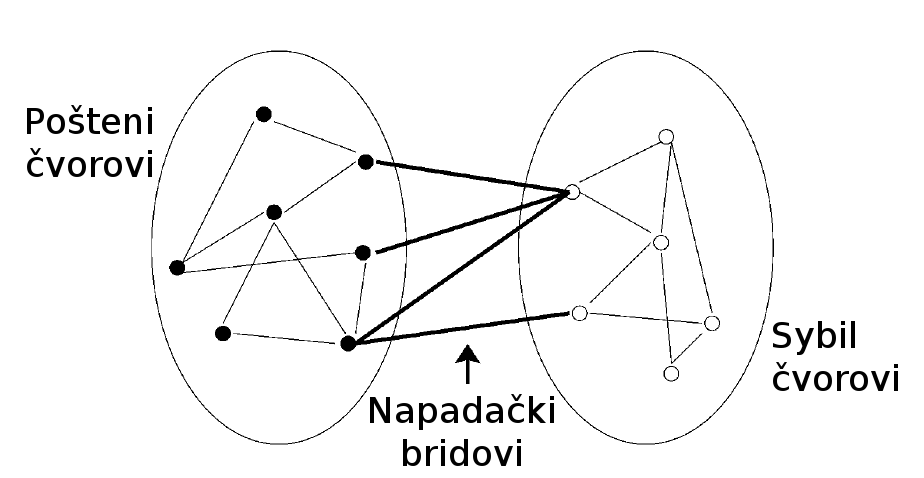
\includegraphics[scale=0.3]{attack.png}
  \end{figure}
\end{frame}

\begin{frame}{Slučajne šetnje}
  \begin{itemize}
    \item \textit{slučajna šetnja} -- šetnja u grafu s nasumično odabranim prijelazima
    \item slučajne šetnje su \textit{ergodične} -- konvergiraju prema \textit{stacionarnoj distribuciji} kada im duljina teži u beskonačnost
  \end{itemize}
\end{frame}

\begin{frame}{Vrijeme miješanja}
  \begin{itemize}
    \item definira se kao najmanja duljina slučajne šetnje kojom se postiže stacionarna distribucija do neke mjere $\epsilon$:
      \[ T(\epsilon) = \max_{i} \min \{t : |\pi - \pi^{(i)} P^t|_1 < \epsilon\} \]
    \item graf s $n$ čvorova je \textit{brzo miješajući} ako je:
      \[ T(\epsilon) = O(\log n) \]
    \item dobro povezani grafovi su brzo miješajući
  \end{itemize}
\end{frame}

\section{Obrana od sybil napada}

\begin{frame}{Pretpostavke algoritma}
  \begin{itemize}
    \item poštena regija je brzo miješajuća
    \item jedan poznat pošteni čvor
    \item administratoru je poznata topologija društvene mreže
    \item veličina sybil regije nije usporediva s veličinom poštene regije
    \item broj napadačkih bridova je ograničen
  \end{itemize}
\end{frame}

\begin{frame}{Identifikacija sybil čvorova: prva faza}
  \begin{itemize}
    \item rade se slučajne šetnje od poznatog poštenog čvora
    \item konačni čvorovi šetnji podvrgavaju se stacionarnoj distribuciji i s visokom su vjerojatnošću pošteni
    \item početni pošteni čvor i dobiveni konačni čvorovi su \textit{čvorovi sudci}
    \item iz svakog od njih napravi se veći broj šetnji različitih duljina
    \item za svaku duljinu pamti se broj čvorova s frekvencijom većom od nekog praga
  \end{itemize}
\end{frame}

\begin{frame}{Identifikacija sybil čvorova: druga faza}
  \begin{itemize}
    \item napravi se veći broj šetnji određene duljine iz \textit{osumljičenog čvora}
    \item izračuna se broj čvorova čija je frekvencija veća od praga
    \item ako je dobiveni broj dovoljno manji od broja izračunatog u prvom koraku za odgovarajuću duljinu, čvor je sybil čvor
    \item u suprotnom postupak, povećava se duljina šetnje i postpuak se ponavlja
    \item ako se dođe do gornje granice za duljinu šetnje, čvor je pošten
  \end{itemize}
\end{frame}

\begin{frame}{Pronalazak sybil grupa: prva faza}
  \begin{itemize}
    \item \textit{mrtva šetnja} je ona koja ponovo prolazi već prijeđenim čvorom
    \item rez između sybil i poštene regije je mali -- ako je duljina šetnje dovoljno velika, omjer mrtvih šetnji biti će blizak 1
    \item u prvoj se fazi određuje duljina šetnje kako bi skup šetnji pokrio barem sybil grupu
  \end{itemize}
\end{frame}

\begin{frame}{Pronalazak sybil grupa: druga faza}
  \begin{itemize}
    \item zadaća druge faze je uklanjanje poštenih čvorova iz nađene sybil grupe
    \item \textit{provodljivost} podgrafa -- omjer broja bridova koji ga spajaju s ostatkom grafa i bridova u njemu
    \item čvorovi se u dobivenoj grupi sortiraju silazno po frekvenciji i višestrukim se iteracijama dodaju sve dok se provodljivost smanjuje
  \end{itemize}
\end{frame}

\section{Rezultati}

\begin{frame}{Korištene metode i skupovi podataka}
  \begin{itemize}
    \item stvarni skupovi podataka iz društvenih mreža Facebook i Orkut s preko 3 milijuna čvorova
    \item dva modela stvaranja sybil regija -- \textit{preferencijalno vezivanje} (PA) i \textit{Erdös-Rényi} (ER)
    \item PA je model s "prirodnom" zastupljenošću stupnjeva čvorova, a ER je potpuno nasumičan
    \item stvorene sybil regije imale su 10,000 čvorova i 1,000 napadačkih bridova
  \end{itemize}
\end{frame}

\begin{frame}{Rezultati}
  \begin{table}
    \centering
    \begin{tabular}{|c|c|c|c|c|c|c|c|c|} \hline
      \multirow{3}{*}{R} & \multicolumn{4}{c|}{Orkut} & \multicolumn{4}{c|}{Facebook} \\
      & \multicolumn{2}{c}{PA model} & \multicolumn{2}{c|}{ER model} & \multicolumn{2}{c}{PA model} & \multicolumn{2}{c|}{ER model} \\
      & \multicolumn{1}{c}{$F^+$} & \multicolumn{1}{c}{$F^-$} & \multicolumn{1}{c}{$F^+$} & \multicolumn{1}{c|}{$F^-$} & \multicolumn{1}{c}{$F^+$} & \multicolumn{1}{c}{$F^-$} & \multicolumn{1}{c}{$F^+$} & \multicolumn{1}{c|}{$F^-$} \\ \hline
      1000 & 0 & 0.02\% & 0 & 0.28\% & 0 & 0.22\% & 0.1\% & 0.54\% \\
      1500 & 0 & 0.02\% & 0 & 0.32\% & 0.3\% & 0.12\% & 0.2\% & 0.44\% \\
      2000 & 0 & 0 & 0 & 0.22\% & 0.5\% & 0.04\% & 0.5\% & 0.4\% \\
      \hline
    \end{tabular}
  \end{table}
\end{frame}

\section{Zaključak}

\begin{frame}{Zaključak}
  \begin{itemize}
    \item algoritam za obranu od sybil napada temeljen na slučajnim šetnjama i algoritamskim svojstvima grafova
    \item identifikacija sybil čvorova i pronalazak grupa koje ih okružuju
    \item algoritam se pokazao veoma učinkovitim i brzim prilikom testiranja na skupovima podataka iz stvarnog svijeta
  \end{itemize}
\end{frame}

\begin{frame}[standout]
  \Huge{\centerline{Pitanja?}}
\end{frame}

\begin{frame}[standout]
  \Huge{\centerline{Hvala na pažnji!}}
\end{frame}

\end{document}
